%!TEX encoding = UTF-8 Unicode
%!TEX root = ../lect-w09.tex

\Subsection{Repetition: sekvens}

\begin{Slide}{Repetition: Vad är en sekvens?}
\begin{itemize}
\item En sekvens är en \Emph{följd av element} som
  \begin{itemize}
   \item är \Alert{numrerade} (t.ex. från noll), och
   \item är av en viss \Alert{typ} (t.ex. heltal).
  \end{itemize}
  \pause
\item En sekvens kan innehålla \Alert{dubbletter}.
\item En sekvens kan vara \Alert{tom} och ha längden noll.
\item Exempel på en icke-tom sekvens med dubbletter:
\begin{REPLnonum}
scala> val xs = Vector(42, 0, 42, -9, 0, 13, 7)
xs: scala.collection.immutable.Vector[Int] =
  Vector(42, 0, 42, -9, 0, 13, 7)
\end{REPLnonum}
\pause
\item \Emph{Indexering} ger ett element via dess ordningsnummer:
\begin{REPL}
scala> xs(2)
res0: Int = 42

scala> xs.apply(2)
res1: Int = 42
\end{REPL}
\end{itemize}
\end{Slide}




\Subsection{Mängd} %%%%%%%%%%%%%%%%%%%%%%%%%%%%%%%%%%%%%%%%%%%%%%%%%%%%%%


\begin{Slide}{Vad är en mängd?}\SlideFontSmall
\begin{itemize}
\item En \Emph{mängd} är en samling \Alert{unika} element av en viss \Alert{typ}.
\item En mängd kan alltså inte innehålla dubbletter:
\begin{REPLnonum}
scala> Set(1,1,2,2,3,3,4,4,5,5)
res0: scala.collection.immutable.Set[Int] =
  Set(5, 1, 2, 3, 4)
\end{REPLnonum}
\pause
\item En mängd är \Alert{inte}  en sekvens: du kan inte utgå från att elementen ligger i någon viss ordning, t.ex. den ordning som de ges vid konstruktion; en mängd har ej längd, men en \Emph{storlek}; metoden \code{size} ger antalet element men metoden \code{length} saknas.
\item Det går således \Alert{inte att indexera} i en mängd.
\item Men man \Emph{kan} gå igenom element i \Emph{någon} ordning (exakt vilken är ej def.), med till exempel \code{xs.map(f)} eller \code{for (x <- xs) yield f(x)}
\item En mängd kan vara \Alert{tom} och har då storleken \code{0}.
\pause
\item En mängd \code{Set[T]} med element av typen \code{T} kan ses som ett \Emph{predikat för innehållstest}: alltså en funktion \code{T => Boolean} som är \code{true} om elementet finns annars \code{false}
\end{itemize}
\end{Slide}


\begin{Slide}{Exempel: Oföränderlig mängd}
\setlength{\leftmargini}{1em}
\begin{itemize}
\item \Emph{Skapa}:
\begin{REPLnonum}
scala> var xs = Set("gurka", "tomat", "banan", "pingvin")
\end{REPLnonum}

\item \Emph{Läsa}: avgöra medlemskap
\begin{REPLnonum}
scala> xs("gurka")
res1: Boolean = true
\end{REPLnonum}

\item \Emph{Uppdatera}: lägg till element (händer inget om redan finns)
\begin{REPLnonum}
scala> xs = xs + "jordekorre"
\end{REPLnonum}

\item \Emph{Ta bort}: (om finns, annars händer inget)
\begin{REPLnonum}
scala> xs = xs - "gurka"
\end{REPLnonum}
\end{itemize}
{\SlideFontTiny\code{SLUT} = Skapa, Läsa, Uppdatera, Ta bort \hfill\code{CRUD} = Create, Read, Update, Delete}
\end{Slide}


\begin{Slide}{Mysteriet med de försvunna elementen}
Vad händer här?
\begin{REPLnonum}
scala> val xs1 = Vector(1,2,3,4,5,6)
scala> xs1.map(_ % 2).count(_ == 0)
res0: Int = 3                          // antalet jämna tal
scala> val xs2 = Set(1,2,3,4,5,6)
scala> xs2.map(_ % 2).count(_ == 0)
res1: Int = 1                          // varför?
\end{REPLnonum}
\pause
Mängdegenskaper ger att \code{xs2.map(_ % 2) == Set(0, 1)}\\
Fundera alltid noga på om du \Alert{riskerar att förlora duplikat} som du egentligen hade velat behålla!\\
\pause
Använd \code{toSeq} på mängd om du behöver sekvensegenskaper:
\begin{REPLnonum}
scala> xs2.toSeq.map(_ % 2).count(_ == 0)
res1: Int = 3         // med toSeq blir det som vi ville
\end{REPLnonum}

\end{Slide}
  
  




\begin{Slide}{Exempel: Förändringsbar mängd}\SlideFontSmall
Med en \Alert{förändringsbar} mängd kan man stegvis utöka på plats.
\begin{REPL}
scala> val mängd = scala.collection.mutable.Set.empty[Int]

scala> for (i <- 1 to 1000000) mängd += i

scala> mängd.contains(-1)                     // samma som mängd(-1)
\end{REPL}
En \Emph{mängd} är \Alert{snabb} på att avgöra om ett element \Alert{finns eller inte} i mängden. Ingen linjärsökning krävs eftersom den smarta implementationen av datastrukturen medger snabb uppslagning \Eng{lookup} av ett element.
\pause
\\\vspace{0.5em}Men i en sekvens krävs linjärsökning vid innehållstest:
\begin{REPL}
scala> val sekvens = (1 to 1000000).toVector

scala> sekvens.contains(-1)   // kräver linjärsökning ända till slutet
\end{REPL}
\pause\SlideFontTiny Övning: Testa själv att mäta tidsskillnaden med hjälp av:
\begin{Code}
def nanos(b: => Unit) = { val t1 = System.nanoTime; b; System.nanoTime - t1 }
\end{Code}

\end{Slide}






\Subsection{Nyckel-värde-tabell} %%%%%%%%%%%%%%%%%%%%%%%%%%%%%%%%%%%%%%%%


\begin{Slide}{Vad är en nyckel-värde-tabell?}\SlideFontSmall
\begin{itemize}
\item En \Emph{nyckel-värde-tabell} är en samling element som är \Alert{par} med:\\
en \Emph{nyckel} av någon typ \code{K} och ett \Emph{värde} av någon typ \code{V}.
\item En sådan tabell kan skapas ur en sekvens av par \code{(k, v)}\\
där \code{k} är en nyckel och \code{v} är ett värde:
\begin{REPL}
scala> val ålder = Map("Björn" -> 42, "Sandra" -> 35, "Kim" -> 19)
ålder: scala.collection.immutable.Map[String,Int] =
  Map(Björn -> 42, Sandra -> 35, Kim -> 19)
\end{REPL}
\item Tabellens nycklar utgör en mängd som ges av metoden \code{keySet};\\
nycklarna är alltså \Alert{unika}.
\item Elementen utgör \Alert{inte en sekvens} och har ingen speciell ordning;
\\en nyckel-värde-tabell har ej längd, men en \Emph{storlek};\\metoden \code{size} ger antalet element.
\pause
\item En tabell kan ses som en uppslagsfunktion \Eng{dictionary}:\\alltså en funktion \code{K => V} som ger ett värde givet en nyckel.
\end{itemize}
\end{Slide}

%
% \begin{Slide}{Exempel: Nyckel-värde-tabell \TODO}
% \setlength{\leftmargini}{1em}
% \begin{itemize}
% \item \Emph{Skapa}:
% \begin{REPLnonum}
% scala> var xs = ???
% \end{REPLnonum}
%
% \item \Emph{Läsa}: slå upp värde utifrån nyckel
% \begin{REPLnonum}
% scala> xs("gurka")
% \end{REPLnonum}
%
% \item \Emph{Uppdatera}: lägg till mappning (händer inget om redan finns)
% \begin{REPLnonum}
% scala> xs = ???
% \end{REPLnonum}
%
% \item \Emph{Ta bort}: ny tabell utan mappning (om finns, annars händer inget)
% \begin{REPLnonum}
% scala> xs = xs - ???
% \end{REPLnonum}
% \end{itemize}
% {\SlideFontTiny\code{SLUT} = Skapa, Läsa, Uppdatera, Ta bort \hfill\code{CRUD} = Create, Read, Update, Delete}
% \end{Slide}




\begin{Slide}{Den fantastiska nyckel-värde-tabellen \texttt{Map}}\SlideFontSmall
\begin{itemize}
\item En \Emph{nyckel-värde-tabell} \Eng{key-value table} är en slags generaliserad vektor där man kan ''indexera'' med godtycklig typ.

\item Kallas även \href{https://sv.wikipedia.org/wiki/Hashtabell}{\Emph{hashtabell}} \Eng{hash table}, \Emph{lexikon} \Eng{dictionary} eller \Emph{mapp} \Eng{map} (men då blir det lätt sammanblandning med metoden \code{map}).

\item Om man vet nyckeln kan man slå upp värdet \Alert{snabbt}, på liknande sätt som indexering sker i en vektor om man vet heltalsindex.

\item Denna datastruktur är \Alert{mycket användbar} och fungerar som en slags databas i kombination med filtrering, registrering, etc.
\end{itemize}
\begin{REPL}
scala> val födelse = Map("C" -> 1972,  "C++" -> 1983, "C#" -> 2000,
  "Scala" -> 2004, "Java" -> 1995, "Javascript" -> 1995, "Python" -> 1991)

scala> födelse.apply("Scala")
res0: Int = 2004

scala> födelse("Java")
res1: Int = 1995
\end{REPL}
Övning: filtrera ut de språk ovan som kom till efter 1999.
\end{Slide}

\begin{Slide}{Exempel nyckel-värde-tabell}\SlideFontSmall
Några ofta förekommande metoder på tabeller:
\begin{itemize}
\item \code{xs.keySet} ger en mängd av alla nycklar
\item \code{xs.map(f)} mappar funktionen f på alla par av (key, value)
\item \code{xs.map(p => p._1 -> f(p._2))} mappar funktionen f på alla värden
\end{itemize}
\begin{REPL}
scala> val färg = Map("gurka" -> "grön", "tomat"->"röd", "aubergine"->"lila")
färg: scala.collection.immutable.Map[String,String] =
  Map(gurka -> grön, tomat -> röd, aubergine -> lila)

scala> färg("gurka")
res0: String = grön

scala> färg.keySet
res1: scala.collection.immutable.Set[String] = Set(gurka, tomat, aubergine)

scala> val ärGrönSak = färg.map(elem => (elem._1, elem._2 == "grön"))
ärGrönSak: Map[String,Boolean] = Map(gurka -> true, tomat -> false, aubergine -> false)

scala> val baklängesFärg = färg.map(p => p._1 -> p._2.reverse)
baklängesFärg: Map[String,String] = Map(gurka -> nörg, tomat -> dör, aubergine -> alil)

\end{REPL}

\end{Slide}



\Subsection{\texttt{scala.collection}} %%%%%%%%%%%%%%%%%%%%%%%%%%%%%%%%%%%



% \begin{Slide}{Typparameter möjliggör generiska samlingar}\SlideFontSmall
%
% \begin{itemize}
%   \item Med \Emph{generisk} \Eng{generic} kod menar man att koden kan hantera data av \Alert{godtycklig} typ.
%   \item Funktioner och klasser kan, förutom vanliga parametrar, även ha \Emph{typparametrar} som skrivs i en \Alert{egen} parameterlista med \Alert{hakparenteser} i stället för vanliga parenteser.
%
%   \item En typparameter gör så att funktioner och datastrukturer blir \Emph{generiska}.
%
%   \item Exempel: Funktionerna \code{baklänges} 1--4 nedan är ordnade från specifik typ till mer generell typ.
%
% \begin{Code}
% def baklänges1(xs: Vector[Int]): Vector[Int] = xs.reverse
%
% def baklänges2[T](xs: Vector[T]): Vector[T] = xs.reverse
%
% def baklänges3(xs: Seq[T]): Vector[T] = xs.reverse.toVector
%
% def baklänges4(xs: Seq[T]): Seq[T] = xs.reverse  //reverse avgör samling
% \end{Code}
% \item Mer om typparametrar i w08.
% \end{itemize}
% \end{Slide}



\begin{Slide}{Hierarki av samlingstyper i \texttt{scala.collection} v2.13}

\begin{multicols}{2}
\begin{tikzpicture}[sibling distance=5.0em,->,>=stealth', inner sep=3pt, %scale=0.5,
  every node/.style = {shape=rectangle, draw, align=center,font=\small\ttfamily},
  class/.style = {fill=blue!20},
  trait/.style = {rounded corners, fill=red!20}]
  \node[trait] {Iterable}
      child { node[trait] {Seq} }
      child { node[trait] {Set} }
      child { node[trait] {Map} }
  ;
\end{tikzpicture}

\columnbreak

{\SlideFontTiny

\code{Iterable} har metoder som är implementerade med hjälp av: \\
\code{def foreach[U](f: Elem => U): Unit}\\
\code{def iterator: Iterator[A] }

}

\begin{itemize}\SlideFontTiny
\item[] \code{Seq}: ordnade i sekvens
\item[] \code{Set}: unika element
\item[] \code{Map}: par av (nyckel, värde)
\end{itemize}


\end{multicols}

{\SlideFontSmall Samlingen \Emph{\texttt{Vector}} är en \code{Seq} som är en \code{Iterable}. \\ \vspace{0.5em}%\pause
De konkreta samlingarna är uppdelade i dessa paket:\\
\code{scala.collection.immutable} \hfill som är \Emph{automatiskt} importerade\\
\code{scala.collection.mutable}  \hfill som \Alert{måste importeras} explicit\\%\pause
(undantag: primitiva \code{scala.Array} som är automatiskt synlig)
}
\end{Slide}




\begin{Slide}{Använda \texttt{iterator} -- primitiv loop över element}\SlideFontSmall
Med en \code{iterator} kan man \Emph{iterera} med \code{while} över alla element, men endast \Alert{en   gång}; sedan är iteratorn ''förbrukad''. (Men man kan be om en ny.)
\begin{REPL}
scala> val xs = Vector(1,2,3,4)
xs: scala.collection.immutable.Vector[Int] = Vector(1, 2, 3, 4)

scala> val it = xs.iterator
it: scala.collection.immutable.VectorIterator[Int] = non-empty iterator

scala> while (it.hasNext) print(it.next)
1234

scala> it.hasNext
res1: Boolean = false

scala> it.next
java.util.NoSuchElementException: reached iterator end
  at scala.collection.immutable.VectorIterator.next(Vector.scala:674)
\end{REPL}
\Emph{Normalt} behöver man \Alert{inte} använda \code{iterator}: det finns oftast färdiga metoder som gör det man vill, till exempel \code{foreach}, \code{map}, \code{sum}, \code{min} etc.
\end{Slide}






% \ifkompendium
% \else
% \begin{Slide}{Hierarki av samlingar i scala.collection v2.12}\SlideFontTiny
% 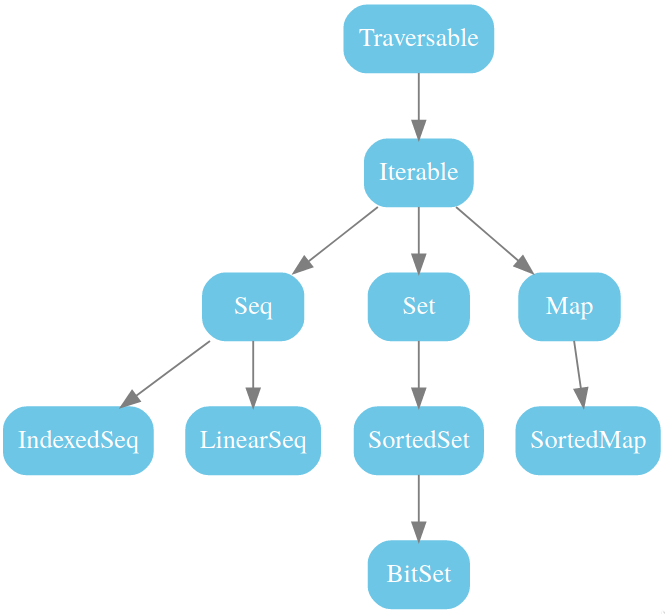
\includegraphics[width=0.6\textwidth]{../img/collection/collection-traits}\\
% %\noindent Läs mer om Scalas samlingar här: \\
% \url{https://docs.scala-lang.org/overviews/collections/overview.html}
% \end{Slide}
% \fi





\begin{Slide}{Mer specifika samlingstyper i \texttt{scala.collection}}
Det finns \Alert{mer specifika} \Emph{subtyper} av \code{Seq}, \code{Set} och \code{Map}:
\\ \vspace{1em}

\begin{tikzpicture}[sibling distance=5.8em,->,>=stealth', inner sep=3pt, %scale=0.5,
  every node/.style = {shape=rectangle, draw, align=center,font=\small\ttfamily},
  class/.style = {fill=blue!20},
  trait/.style = {rounded corners, fill=red!20}]
  \node[trait] {Iterable}
      child { node[trait, xshift=-2.4cm] {Seq}
        child { node[trait] {IndexedSeq} }
        child { node[trait] {LinearSeq} }
       }
      child { node[trait, yshift=-0.0cm] {Set}
        child { node[trait] {SortedSet} }
        child { node[trait] {BitSet} }
      }
      child { node[trait, xshift=1.0cm] {Map}
        child { node[trait] {SortedMap} }
    };
\end{tikzpicture}

\pause\vspace{0.5em}
\Emph{\texttt{Vector}} är en \Alert{\texttt{IndexedSeq}} medan
\Emph{\texttt{List}} är en \Alert{\texttt{LinearSeq}}.

\pause\vspace{1em}{\SlideFontSmall
\href
{https://docs.scala-lang.org/overviews/collections-2.13/overview.html}
{docs.scala-lang.org/overviews/collections-2.13/overview.html}
}
\end{Slide}

\begin{Slide}{Några oföränderliga och förändringsbara sekvenssamlingar}\SlideFontSmall
\begin{tabular}{r l l}
\texttt{scala.collection.\Emph{immutable}.Seq.} & & \\
 & \code|IndexedSeq.| & \\
 & & \Emph{\texttt{Vector}} \\
 & & \Emph{\texttt{Range}} \\
 & \code|LinearSeq.| & \\
 & & \Emph{\texttt{List}} \\
   & & \Emph{\texttt{Queue}} \\

\texttt{scala.collection.\Alert{mutable}.Seq.} & & \\
 & \code|IndexedSeq.| & \\
 & & \Alert{\texttt{ArrayBuffer}} \\
 & & \Alert{\texttt{StringBuilder}} \\
 & \code|LinearSeq.| & \\
 & & \Alert{\texttt{ListBuffer}} \\
   & & \Alert{\texttt{Queue}} \\
\end{tabular}

Fördjupning: Studera samlingars prestandaegenskaper här:\\ \href{https://docs.scala-lang.org/overviews/collections/performance-characteristics.html}{docs.scala-lang.org/overviews/collections/performance-characteristics.html}
\end{Slide}



\begin{Slide}{Några användbara metoder på samlingar}\SlideFontTiny
\begin{tabular}{r r l}\hline
\texttt{\Emph{Iterable}}
  & \code|xs.size| & antal elementet \\
  & \code|xs.head| & första elementet \\
  & \code|xs.last| & sista elementet \\
  & \code|xs.take(n)| & ny samling med de första n elementet \\
  & \code|xs.drop(n)| & ny samling utan de första n elementet \\
  & \code|xs.foreach(f)| & gör \code|f| på alla element, returtyp \code|Unit|\\
  & \code|xs.map(f)| & gör \code|f| på alla element, ger ny samling \\
  & \code|xs.filter(p)| & ny samling med bara de element där p är sant\\
  & \code|xs.groupBy(f)| & ger en \code|Map| som grupperar värdena enligt f\\
  & \code|xs.mkString(",")| & en kommaseparerad sträng med alla element\\ 
  & \code|xs.zip(ys)| & ny samling med par (x, y); ''zippa ihop'' xs och ys \\
  & \code|xs.zipWithIndex| & ger en \code|Map| med par (x, index för x) \\
  & \code|xs.sliding(n)| & ny samling av samlingar genom glidande ''fönster''\\ \hline

\texttt{\Emph{Seq}}
  & \code|xs.length| & samma som \code|xs.size| \\
  & \code|xs :+ x| & ny samling med x sist efter xs \\
  & \code|x +: xs| & ny samling med x före xs \\ \hline

\end{tabular}

\pause
\vspace{0.5em}\Emph{Minnesregel} för \code{+:} och \code{:+  } \pause \Alert{Colon on the collection side}

\pause
Prova fler samlingsmetoder ur snabbreferensen: ~~\url{http://cs.lth.se/quickref}
\end{Slide}



\begin{Slide}{Från sekvens av par till tabell}
\begin{REPL}
scala> val xs = Vector(("Kim",42), ("Pam", 42), ("Kim", 50), ("Pam", 50))

xs: Vector[(String, Int)] =
  Vector((Kim,42), (Pam,42), (Kim,50), (Pam,50))


scala> xs.toMap

res0: Map[String,Int] = Map(Kim -> 50, Pam -> 50)  // inga dublettnycklar


scala> val grupperaEfterNamn = xs.groupBy(_._1)

grupperaEfterNamn: Map[String,Vector[(String, Int)]] =
  Map(Kim -> Vector((Kim,42), (Kim,50)), Pam -> Vector((Pam,42), (Pam,50)))


scala> val grupperaEfterÅlder = xs.groupBy(_._2)

grupperaEfterÅlder: Map[Int,Vector[(String, Int)]] =
  Map(50 -> Vector((Kim,50), (Pam,50)), 42 -> Vector((Kim,42), (Pam,42)))
\end{REPL}
\end{Slide}



\begin{Slide}{Metoderna zipWithIndex, groupBy}
\vspace{-0.5em}
\begin{REPL}
scala> val kort = Vector("Knekt", "Dam", "Kung", "Äss")

scala> val kortIndex = kort.zipWithIndex.toMap
kortIndex: Map[String,Int] = Map(Knekt -> 0, Dam -> 1, Kung -> 2, Äss -> 3)

scala> kortIndex("Kung") > kortIndex("Knekt")
res0: Boolean = true

scala> kortIndex.map(p => p._1 -> (p._2 + 11))

scala> val tärningskast = Vector(1,2,3,4,5,6,2,4,6)

scala> val grupperaStörreÄnFyra = xs.groupBy(_ > 4)
grupperaStörreÄnFyra: Map[Boolean,Vector[Int]] =
  Map(false -> Vector(1, 2, 3, 4, 2, 4), true -> Vector(5, 6, 6))

scala> val grupperaLika = xs.groupBy(x => x)
grupperaLika: Map[Int,Vector[Int]] = Map(5 -> Vector(5), 1 -> Vector(1),
  6 -> Vector(6, 6), 2 -> Vector(2, 2), 3 -> Vector(3), 4 -> Vector(4, 4))

scala> val frekvens = tärningskast.groupBy(x => x).map(p => p._1 -> p._2.size)
frekvens: Map[Int,Int] = Map(5 -> 1, 1 -> 1, 6 -> 2, 2 -> 2, 3 -> 1, 4 -> 2)

\end{REPL}
\end{Slide}


% \ifkompendium\else

% \begin{Slide}{scala.collection.immutable}
% 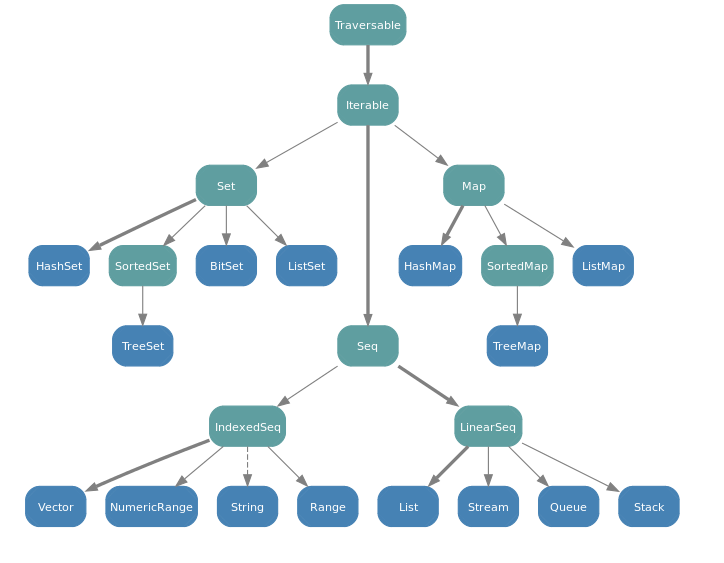
\includegraphics[width=0.67\textwidth]{../img/collection/collection-immutable}~~%
% 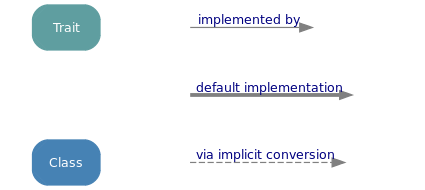
\includegraphics[width=0.3\textwidth]{../img/collection/collection-legend}
% \end{Slide}


% \begin{Slide}{scala.collection.mutable}
% 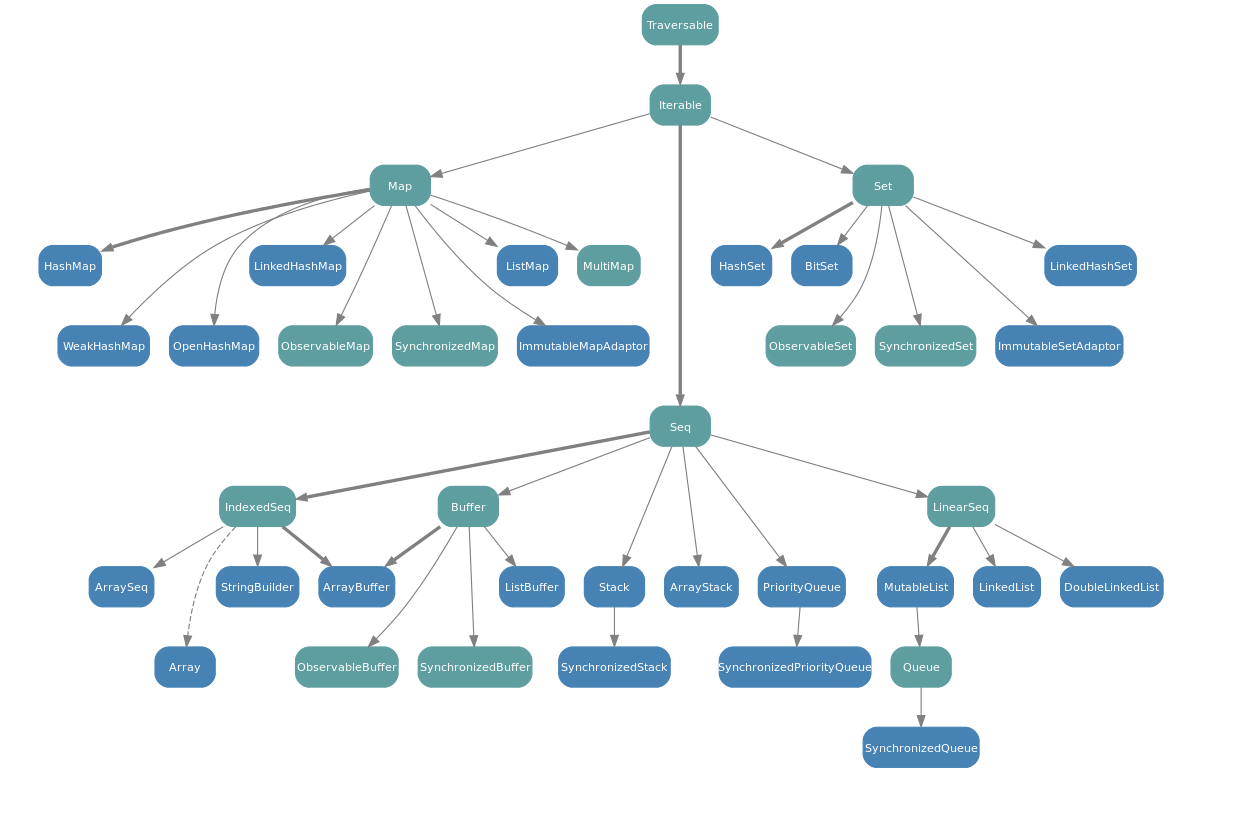
\includegraphics[width=1.05\textwidth]{../img/collection/collection-mutable}
% \end{Slide}

% \fi

\begin{Slide}{Strängar är implicit en \texttt{IndexedSeq[Char]}}\SlideFontSmall
Det finns en så kallad \Emph{implicit konvertering} mellan \code{String} och \code{IndexedSeq[Char]} vilket gör att \Alert{alla samlingsmetoder på \texttt{Seq} även funkar på strängar} och även flera andra smidiga strängmetoder erbjuds \Alert{utöver} de som finns i \href{http://docs.oracle.com/javase/8/docs/api/java/lang/String.html}{\code{java.lang.String}} genom klassen \href{http://www.scala-lang.org/api/current/scala/collection/immutable/StringOps.html}{\code{StringOps}}.

\vspace{0.5em}
\begin{REPLnonum}
scala> "hej".  //tryck på TAB och se alla strängmetoder
\end{REPLnonum}
Detta är en stor fördel med Scala jämfört med många andra språk, som har strängar som inte kan allt som andra sekvenssamlingar kan.
\end{Slide}


% \begin{Slide}{\texttt{Vector} eller \texttt{List}?}\SlideFontTiny
% {\href{http://stackoverflow.com/questions/6928327/when-should-i-choose-vector-in-scala}{stackoverflow.com/questions/6928327/when-should-i-choose-vector-in-scala}}
%
% \begin{enumerate}
% \item If we only need to transform sequences by operations like map, filter, fold etc: basically it does not matter, we should program our algorithm generically and might even benefit from accepting parallel sequences. For sequential operations List is probably a bit faster. But you should benchmark it if you have to optimize.
%
% \item If we need a lot of random access and different updates, so we should use vector, list will be prohibitively slow.
%
% \item If we operate on lists in a classical functional way, building them by prepending and iterating by recursive decomposition: use list, vector will be slower by a factor 10-100 or more.
%
% \item If we have an performance critical algorithm that is basically imperative and does a lot of random access on a list, something like in place quick-sort: use an imperative data structure, e.g. ArrayBuffer, locally and copy your data from and to it.
% \end{enumerate}
% {\href{http://stackoverflow.com/questions/20612729/how-does-scalas-vector-work}{stackoverflow.com/questions/20612729/how-does-scalas-vector-work}}\\
% Mer om tids- och minneskomplexitet i fördjupningskursen och senare kurser.
% \end{Slide}




\begin{Slide}{Speciella metoder på förändringsbara samlingar}\SlideFontSmall
Både \code{Set} och \code{Map} finns i \Alert{förändringsbara} varianter med extra metoder för uppdatering av innehållet ''på plats'' utan att nya samlingar skapas.
\begin{REPL}
scala> import scala.collection.mutable

scala> val ms = mutable.Set.empty[Int]
ms: scala.collection.mutable.Set[Int] = Set()

scala> ms += 42
res0: ms.type = Set(42)

scala> ms += (1, 2, 3, 1, 2, 3); ms -= 1
res1: ms.type = Set(2, 42, 3)

scala> ms.mkString("Mängd: ", ", ", " Antal: " + ms.size)
res2: String = Mängd: 1, 2, 42, 3 Antal: 4

scala> val ordpar = mutable.Map.empty[String, String]
scala> ordpar += ("hej" -> "svejs", "abra" -> "kadabra", "ada" -> "lovelace")
scala> println(ordpar("abra"))
kadabra
\end{REPL}
\end{Slide}

\begin{Slide}{Fler exempel på samlingsmetoder}
Exempel att öva på: räkna bokstäver i ord.  \\
Undersök vad som händer i REPL:
\begin{Code}[basicstyle=\SlideFontSize{9}{13}\ttfamily]
val ord = "sex laxar i en laxask sju sjösjuka sjömän"
val uppdelad = ord.split(' ').toVector
val ordlängd = uppdelad.map(_.length)
val ordlängdMap = uppdelad.map(s => (s, s.size)).toMap
val grupperaEfterFörstaBokstav = uppdelad.groupBy(s => s(0))
val bokstäver = ord.toVector.filter(_ != ' ')
val antalX = bokstäver.count(_ == 'x')
val grupperade = bokstäver.groupBy(ch => ch)
val antal = grupperade.map(p => p._1 -> p._2.size)
val sorterat = antal.toVector.sortBy(_._2)
val vanligast = antal.maxBy(_._2)
\end{Code}
\end{Slide}


\begin{Slide}{Föränderlig lokalt, returnera oföränderlig}
\SlideFontSmall
Om du vill implementera en imperativ algoritm med en föränderlig samling:\\
Gör gärna detta \Alert{lokalt} i en \Alert{förändringsbar} samling och returnera sedan en \Emph{oföränderlig} samling, genom att köra t.ex. \code{toSet} på en mängd, eller \code{toMap} på en hashtabell, eller \code{toVector} på en \code{ArrayBuffer} eller \code{Array}.

\begin{REPL}
scala> :paste
def kastaTärningTillsAllaUtfallUtomEtt(sidor: Int = 6) = {
  val s = scala.collection.mutable.Set.empty[Int]
  var n = 0
  while (s.size < sidor - 1) {
    s += (math.random() * sidor + 1).toInt
    n += 1
  }
  (n, s.toSet)
}
scala> kastaTärningTillsAllaUtfallUtomEtt()
res0: (Int, scala.collection.immutable.Set[Int]) = (13,Set(5, 1, 6, 2, 3))

\end{REPL}
\end{Slide}


\begin{Slide}{Metoden \texttt{sliding}}\SlideFontSmall
Metoden \code{sliding(n)} skapar med ett ''glidande fönster'' en sekvens av
delsekvenser av längd \code{n} genom att ''svepa fönstret'' från början till slut:
\begin{REPL}
scala> val xs = "fem myror är fler än fyra elefanter".split(' ').toVector
xs: Vector[String] = Vector(fem, myror, är, fler, än, fyra, elefanter)

scala> xs.sliding(2).toVector
res0: Vector[Vector[String]] =
  Vector(Vector(fem, myror), Vector(myror, är), Vector(är, fler),
     Vector(fler, än), Vector(än, fyra), Vector(fyra, elefanter))

scala> xs.sliding(3).toVector
res1: Vector[Vector[String]] =
  Vector(Vector(fem, myror, är), Vector(myror, är, fler),
    Vector(är, fler, än), Vector(fler, än, fyra),
      Vector(än, fyra, elefanter))
\end{REPL}
Denna metod har du nytta av på veckans laboration!
\\(se fler exempel på övning)
\end{Slide}
